\section{Постановка задачи}
\subsection{Одномерное течение}
\par В этой работе рассматривается одномерное течение жидкости с частицами сквозь пористую среду. Выпишем систему уравнений для одномерного течения:
$$\displaystyle \begin {cases}
(m\alpha)'_{t}+(\alpha u)'_{x}=m'_{t}\\
u'_{x}=0\\
\displaystyle -P'_{x}-\frac{\mu}{k}u=0\\
m_{t}=-f(|\vec{u}|, m, \alpha)\\
\end {cases}$$

\par Сделаем следующие предположения. Пусть скорость $u=u_{0}=const$. Получили следующую систему:\\
$$\begin {cases}
(m\alpha)_{t}+\alpha_{x}u_{0}=m_{t}\\
m_{t}=-f(|\vec{u}|, m, \alpha)
\end{cases}$$
\par Получившаяся в результате предположений система является квазилинейной и содержит две неизвестные.

\subsection{Граничные условия}
\par В задаче рассматриваются следующие граничные условия:
\par \textbf{На входе} в пласт положим заданной концентрацию частиц $\alpha|_{x=0}=\alpha_{0}(t)$ и, в частности, $\alpha_{0}=const$\\
\par В начальный момент времени $t=0$ считаем заданной пористость среды  $m=m_{0},\text{а концентрацию}\;\;\alpha=0$ --- внутри пористой среды первоначально \textbf{чистая} жидкость.\\
\par \textbf{На выходе} из пласта при $x=L$ условия не ставятся, что связано с поведением характеристик.\\
\pagebreak
\subsection{Начало закачки в пласт}
\par На иллюстрации схематически показана зависимость $m$ и $\alpha$ от координаты $x$ в различные моменты времени $t_{i}$:
\begin{figure}[h!]
\center{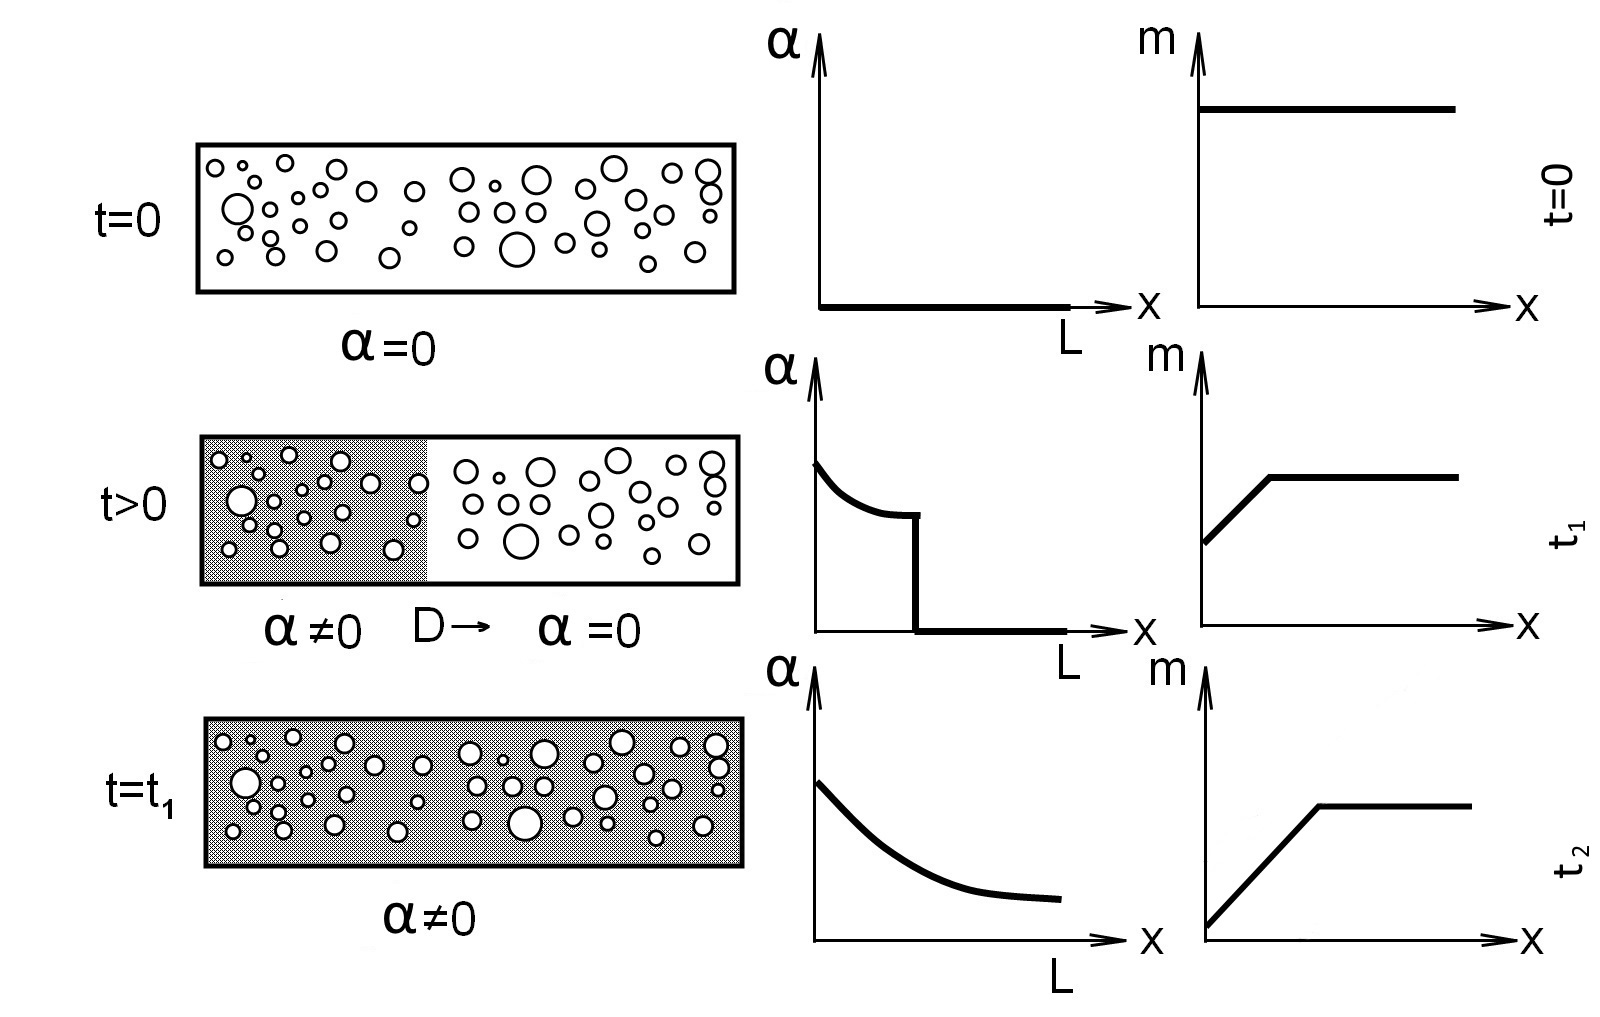
\includegraphics[width=15cm]{begining_of_loading.jpg}}
\caption{}
\label{fig:image1}
\end{figure}